\documentclass{beamer}



%Information to be included in the title page:
\title{\textbf{Detecting changes in dispersion in COVID-19 case counts using a negative binomial model}}
\subtitle{JSM 2024}
\author{Rachael Aber, Yanming Di, Ben Dalziel}
\date{2024}
\logo{
\includegraphics[height=1.5cm]{osu_logo}}

% import citation package
\usepackage[backend=biber]{biblatex}
\addbibresource{references.bib}

\AtBeginSection[]
{
	\begin{frame}
		\frametitle{Table of Contents}
		\tableofcontents[currentsection]
	\end{frame}
}

\begin{document}

\frame{\titlepage}

\begin{frame}
	\frametitle{Table of Contents}
	\tableofcontents
\end{frame}

\section{Why study variability?}
	
\begin{frame}
\frametitle{Why study variability?}
\begin{itemize}[<+-| alert@+>] % other than alert it's also okay to insert \pause manually.
			\item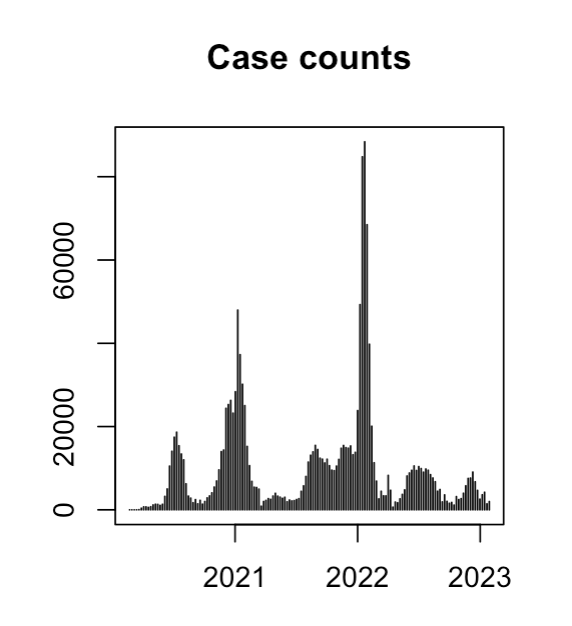
\includegraphics[height=2cm]{var}
			\item Highly variable case count time series suggest transmission heterogeneity, demographic/environmental heterogeneity, or changes in R
			\item Metrics of variability are overlooked (way to): "How is variability related to different phases of an epidemic?"\cite{graham_measles_2019}
			\item Adam et al.\cite{adam_time-varying_2022} found that COVID-19 transmission heterogeneity decreased over time; associated with interventions to slow spread
			\item Information about what phase/dynamic regime an epidemic is in, as well as indicating the level of heterogeneity at finer spatial and temporal scales (in)
	\end{itemize}
\end{frame}

\begin{frame}{\textbf{Why study variability?}}
	\begin{itemize}[<+-| alert@+>] 
		\item Dispersion (around) of a case count time series may be a useful metric--part of a framework that models variance (more) flexibly
		\item A 'mean crowding' parameter \cite{lloyd_mean_1967} was proposed, which is the mean number per individual of other individuals in the same quadrat 
		\item Useful way to think about dispersion in case count time series, degree of dispersion is degree of clustering/crowding of cases (from the perspective)
		\item 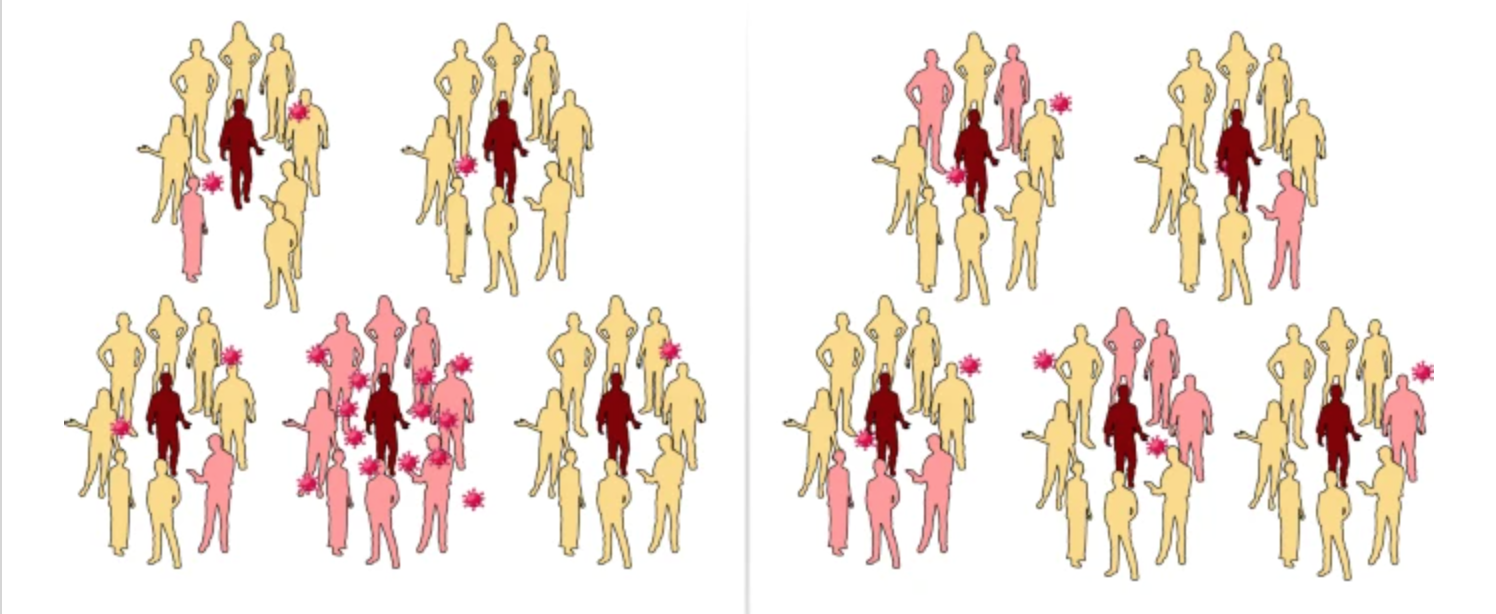
\includegraphics[height=2cm]{sup}
	\end{itemize}
\end{frame}

\section{Negative binomial model}
\begin{frame}{\textbf{Introduction to the method}}
	\begin{itemize}[<+-| alert@+>] 
		\item Let \begin{math}\lambda_t\end{math} 
		\item \begin{equation}
			\mathrm{I_t = NB(\mu = \lambda_t, \theta_t = I_{t-1})}
		\end{equation}
		\item Adjusted for population size using an offset in the model (directly model)
		\item Dispersion allowed to vary more slowly than the process mean
		\item Linear predictor includes a natural spline in time to account for autocorrelation in case counts (ns are)
		\begin{align}
			log(E[Y_i]/n_i) &= \beta_1h_1(t_i) + \beta_2h_2(t_i) + \beta_3h_3(t_i) \\
			log(E[Y_i])-log(n_i) &= \beta_1h_1(t_i) + \beta_2h_2(t_i) + \beta_3h_3(t_i) \\ 
			log(E[Y_i]) &= \beta_1h_1(t_i) + \beta_2h_2(t_i) + \beta_3h_3(t_i) + log(n_i) 
		\end{align}
	\end{itemize}
\end{frame}

\begin{frame}{\textbf{Negative binomial model}}
	\begin{itemize}[<+-| alert@+>] 
		\item \begin{equation}
			f_t(I) = \binom{I + \theta - 1}{I} \frac{\mu}{\mu+\theta}^I \frac{\theta}{\mu +\theta}^\theta
		\end{equation}
		\item \begin{align}
		E(I) &= \mu\\
		Var(I) &= \mu + \frac{\mu^2}{\theta}
	\end{align}
	\item LRT framework with null that dispersion stays the same - applied on a rolling basis
	\end{itemize}
\end{frame}

\begin{frame}{\textbf{Application to simulated data}}
\begin{itemize}[<+-| alert@+>]
	\item For validity/power simulations, we used both Gaussian and uniform epidemic curves with an attack rate of 0.1 
	\item Epidemic curves over 60 timesteps each were produced, and the likelihood-ratio test (LRT) procedure was applied to each
	\item Varying the effect size, location of the breakpoint, population size, and curve shape allowed us to test the validity and power of our approach
\end{itemize}
\end{frame}

\begin{frame}{\textbf{Application to empirical data}}
	\begin{itemize}[<+-| alert@+>]
		\item We estimated \begin{math}\mu_t\end{math} and \begin{math}\theta_t\end{math} using an iterative reweighted least-squares (procedure implemented via the NBPSeq package\cite{NBPSeq} and from Di et al.\cite{yanming_nbp_2011} with a moving window approach (for each window)
		\item We investigated large counties (largest three counties in each state)
	\end{itemize}
\end{frame}

\section{Results}
\begin{frame}{\textbf{Correspondence simulated and empirical}}
	\begin{itemize}[<+-| alert@+>]
		\item We found that the negative binomial/LRT method is robust to differences in population size (for population sizes examined) (for, row)
		\item In row one and two of Fig. 1, we illustrated that an increase in \begin{math}\theta\end{math} is associated with decreased variability in simulated incidence time series  (same relationship is observable in the empirical time series), with an increase in \begin{math}\theta\end{math} corresponding to a decrease in variability around the trend in incidence
	\end{itemize}
\end{frame}

\begin{frame}{\textbf{Correspondence simulated and empirical}}
		\begin{figure}[!h]
			
\includegraphics[width=0.8\textwidth]{fig1}
			\caption{
				Detecting dispersion changes in incidence time series in populations of different sizes. A: Simulated incidence when dispersion is constant. B: When dispersion changes during the epidemic. C: Constant dispersion used in generation of above. D: Changing dispersion used in generation of above. E:  Performance of the method with simulated data that has different absolute differences in theta (horizontal axis of each pane) illustrates p-value distribution across different population sizes (each pane is one population size). O and X mark the null and alternative hypotheses indicated in panels C and D. 
			}
			\label{fig1}
		\end{figure}
\end{frame}

\begin{frame}{\textbf{}}
		\begin{figure}[!h]
			
\includegraphics[width=0.4\textwidth]{compare}
			\caption{
				Method applied to case counts between 2020-01-04 and 2023-03-18 for Jefferson County, AL. A: Case counts . B: LRT statistic C: Log dispersion parameter.
			}
			\label{fig2}
		\end{figure}
\end{frame}

\begin{frame}{\textbf{Applied to counties}}
	\begin{itemize}[<+-| alert@+>]
		\item Highly overdispersed incidence patterns observed more frequently later in time series (consistent) (Most dispersed category in Fig reaches) 
		\item Evidence for a change in \begin{math}\theta\end{math} was observed across many counties (evidenced by concentration of low p-values around peak incidence) 
		\item High dispersion may indicate less diffuse epidemics that are potentially more subject to climate forcing\cite{dalziel_urbanization_2018}, or increased locally experienced mean density \cite{lloyd_mean_1967}
	\end{itemize}
\end{frame}

\begin{frame}{\textbf{Applied to counties}}
	\begin{figure}[!h]
	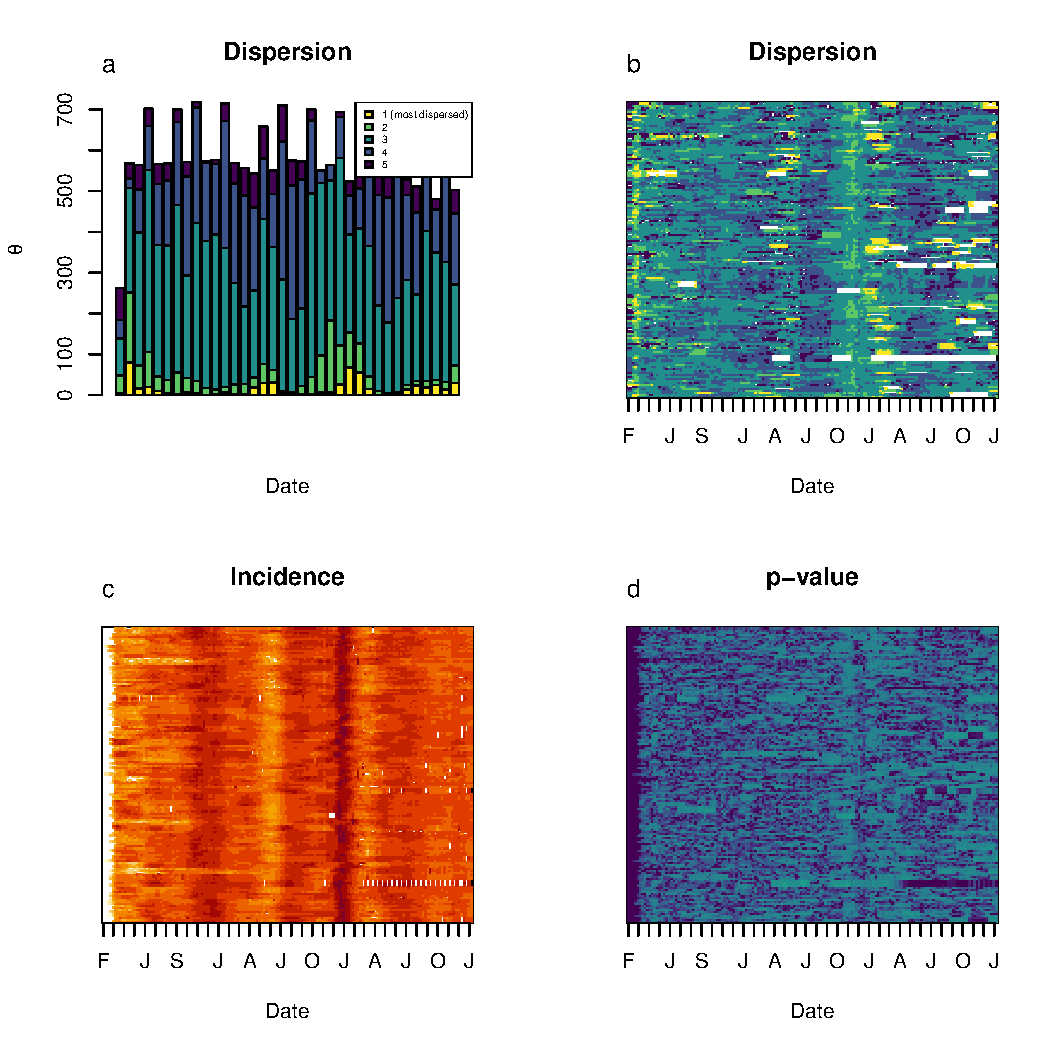
\includegraphics[width=0.4\textwidth]{fig2}
	\caption{
		Incidence and dispersion between 2020-01-04 and 2023-03-18 in large counties in the US. A: Binned log of the dispersion parameter over time. B: Log of the dispersion parameter over time as well as for each of the large counties (y-axis). C: Log incidence (new cases per individual) over time as well as for each of the large counties (y-axis). D: LRT p-values over time as well as for each of the large counties (y-axis).
	}
	\label{fig2}
\end{figure}
\end{frame}

\section{Concluding remarks}
\begin{frame}{\textbf{Concluding remarks}}
	\begin{itemize}[<+-| alert@+>]
		\item Quantify variability in epidemic time series that does not detect artifacts based on population size and incidence (forms)
		\item Methods that use time series are crucial  (due to) 
		\item Timing/allocation of public health resources can be achieved (with) 
		\item Population-wide disease control approaches are often less effective than those which are targeted to individuals in high-transmission contexts \cite{lloyd-smith_superspreading_2005} (catalyze the development of more efficient control strategies)
		\item Our results imply (revise): dispersion is high at unexpected times (near peak incidence)
		\item Raising variance relative to mean implies spatiotemporal "crowding" of cases (i.e. localized surges) which may necessitate more surge capacity in hospitals and testing centers
	\end{itemize}
\end{frame}

\section{References}

\begin{frame}
	\begin{center}
		{\Huge Thanks!}
	\end{center}
\end{frame}

\end{document}